%% For double-blind review submission, w/o CCS and ACM Reference (max submission space)
%\documentclass[sigplan,10pt,review]{acmart}\settopmatter{printfolios=true,printccs=false,printacmref=false}
%
\documentclass[sigplan,10pt]{acmart}\settopmatter{printfolios=true,printccs=false,printacmref=false}
%
%% For double-blind review submission, w/ CCS and ACM Reference
%\documentclass[sigplan,10pt,review,anonymous]{acmart}\settopmatter{printfolios=true}
%% For single-blind review submission, w/o CCS and ACM Reference (max submission space)
%\documentclass[sigplan,10pt,review]{acmart}\settopmatter{printfolios=true,printccs=false,printacmref=false}
%% For single-blind review submission, w/ CCS and ACM Reference
%\documentclass[sigplan,10pt,review]{acmart}\settopmatter{printfolios=true}
%% For final camera-ready submission, w/ required CCS and ACM Reference
%\documentclass[sigplan,10pt]{acmart}\settopmatter{}


%% Conference information
%% Supplied to authors by publisher for camera-ready submission;
%% use defaults for review submission.
\acmConference[PL'17]{ACM SIGPLAN Conference on Programming Languages}{January 01--03, 2017}{New York, NY, USA}
\acmYear{2017}
\acmISBN{} % \acmISBN{978-x-xxxx-xxxx-x/YY/MM}
\acmDOI{} % \acmDOI{10.1145/nnnnnnn.nnnnnnn}
\startPage{1}

%% Copyright information
%% Supplied to authors (based on authors' rights management selection;
%% see authors.acm.org) by publisher for camera-ready submission;
%% use 'none' for review submission.
\setcopyright{none}
%\setcopyright{acmcopyright}
%\setcopyright{acmlicensed}
%\setcopyright{rightsretained}
%\copyrightyear{2017}           %% If different from \acmYear

%% Bibliography style
\bibliographystyle{ACM-Reference-Format}
%% Citation style
%\citestyle{acmauthoryear}  %% For author/year citations
%\citestyle{acmnumeric}     %% For numeric citations
%\setcitestyle{nosort}      %% With 'acmnumeric', to disable automatic
                            %% sorting of references within a single citation;
                            %% e.g., \cite{Smith99,Carpenter05,Baker12}
                            %% rendered as [14,5,2] rather than [2,5,14].
%\setcitesyle{nocompress}   %% With 'acmnumeric', to disable automatic
                            %% compression of sequential references within a
                            %% single citation;
                            %% e.g., \cite{Baker12,Baker14,Baker16}
                            %% rendered as [2,3,4] rather than [2-4].


%%%%%%%%%%%%%%%%%%%%%%%%%%%%%%%%%%%%%%%%%%%%%%%%%%%%%%%%%%%%%%%%%%%%%%
%% Note: Authors migrating a paper from traditional SIGPLAN
%% proceedings format to PACMPL format must update the
%% '\documentclass' and topmatter commands above; see
%% 'acmart-pacmpl-template.tex'.
%%%%%%%%%%%%%%%%%%%%%%%%%%%%%%%%%%%%%%%%%%%%%%%%%%%%%%%%%%%%%%%%%%%%%%


%% Some recommended packages.
\usepackage{booktabs}   %% For formal tables:
                        %% http://ctan.org/pkg/booktabs
\usepackage{subcaption} %% For complex figures with subfigures/subcaptions
                        %% http://ctan.org/pkg/subcaption

\usepackage{graphicx}
\usepackage{graphics}
\usepackage{amsmath,amssymb, amsfonts, mathtools}
\usepackage{isabelle,isabellesym}
\usepackage{listings}

\newcommand{\defeq}{\mathrel{\stackrel{\mbox{\tiny \it def}}{=}}}
\newcommand{\subpred}{\Rightarrow}
%\newcommand{\subpred}{\mathrel{\stackrel{\cdot}{\subseteq}}}
\newcommand{\sconj}{\wedge^*}
\newcommand{\coloncolon}{\mathrel{::}}
\newcommand{\pvalid}[3]{\models\{#1\}\:#2\:\{#3\}}
\newcommand{\tvalid}[3]{\models[#1]\:#2\:[#3]}
\newcommand{\ttrip}[5]{\mathit{#1} \vdash_{\mathrm{#2}}[#3]\:#4\:[#5]}
\newcommand{\xnext}{\mathit{next}}
\newcommand{\code}[1]{\mathit{code}(#1)}
\newcommand{\cont}{\mathit{continuing}}
\newcommand{\ncont}{\mathit{not\mbox{-}continuing}}
\newcommand{\pc}{\mathit{pc}}
\newcommand{\gaspred}{\mathit{gas\mbox{-}pred}}
\newcommand{\stackh}{\mathit{stack\mbox{-}height}}
\newcommand{\stack}{\mathit{stack}}
\newcommand{\storage}{\mathit{storage}}
\newcommand{\instr}[1]{\mathtt{#1}}
\newcommand{\pure}[1]{\langle#1\rangle}
\newcommand{\hd}{\mathit{head}\:}
\newcommand{\RuleL}[2]{\begin{array}{l}#1\\\hline\noalign{\smallskip}#2\end{array}}
\newcommand{\RuleC}[2]{\begin{array}{c}#1\\\hline\noalign{\smallskip}#2\end{array}}
\newcommand{\Rule}[2]{\dfrac{#1}{#2}}
\newcommand{\bblocks}{\mathit{build\mbox{-}blocks}}
\newcommand{\cblocks}{\mathit{connect\mbox{-}blocks}}
\newcommand{\fblock}{\mathit{first\mbox{-}block}}
\newcommand{\len}[1]{|#1|}
\newcommand{\wfblocks}{\mathit{wf\mbox{-}blocks}}

%%%%%%%%%%%%%%%%%%
\newcommand{\sid}[1]{\textit{\textbf{#1 [sid]}}}



% define solidity colorscheme

\lstset{
  basicstyle=\footnotesize,
  commentstyle=\rm\it,
  flexiblecolumns=false,
  breaklines=true,
  breakautoindent=false
}

% possible usage
%\lstinline!apply(simp)!
%\begin{lstlisting}[language=Isar]{}
%datatype type = IntType | BoolType | FunType type type | ErrorType
%\end{lstlisting}
%\lstinputlisting[language=Isar]{foo.thy}

% Taken from Lena Herrmann at 
% http://lenaherrmann.net/2010/05/20/javascript-syntax-highlighting-in-the-latex-listings-package
\definecolor{lightgray}{rgb}{.9,.9,.9}
\definecolor{darkgray}{rgb}{.4,.4,.4}
\definecolor{purple}{rgb}{0.65, 0.12, 0.82}

\lstdefinelanguage{Solidity}{
  keywords={typeof, new, true, false, catch, function, return, null, catch, switch, var, if, in, while, do, else, case, break, returns, contract, public,payable},
  keywordstyle=\color{blue}\bfseries,
  keywordstyle=[2]\color{black}\bfseries,
  keywordstyle=[3]\color{purple}\bfseries,
  keywordstyle=[4]\color{black}\bfseries,
  keywords=[2]{address, uint256},
  keywords=[3]{require,selfdestruct},
  keywords=[4]{address,uint256},
  ndkeywords={class, export, boolean, throw, implements, import, this},
  ndkeywordstyle=\color{black}\bfseries,
  numbers=left,
  numbersep=5pt,
  identifierstyle=\color{black},
  sensitive=false,
  comment=[l]{//},
  morecomment=[s]{/*}{*/},
  commentstyle=\color{purple}\ttfamily,
  stringstyle=\color{red}\ttfamily,
  morestring=[b]',
  morestring=[b]"
}

\lstset{
   extendedchars=true,
   tabsize=2,
   breaklines=true,
   captionpos=b
}

% end define Solidity colorscheme
% define  Isar
\lstdefinelanguage{Isar}%
  {keywords={
        theory,end,types,datatype,consts,defs,primrec,
        syntax,translations,apply,definition,fun,function, lemma,theorem,corollary,
        done,sorry,goal,proof,fixed variables, inductive, where, case,of,if,then,else,method},
        sensitive=true,
        comment=[s]{(*}{*)},
        commentstyle=\color{purple}\ttfamily,
        keywordstyle=\color{blue}\bfseries,
        literate=
                {\\<not>}{{$\<not>$}}1 {\\<times>}{{$\<times>$}}1                 
                {\\<Rightarrow>}{{$\Rightarrow$}}1%
                {\\<models>}{{$\models$}}1%
                {\\<equiv>}{{$\equiv$}}1 {~=}{{$\not=$}}1                         
                {\\<rightleftharpoons>}
                        {{$\rightleftharpoons$}}1
                {\\<exists>}{{$\exists$}}1
                {\\<parallel>}{{$\parallel$}}1
                {\\<Longrightarrow>}
                        {{$\Longrightarrow$}}1
                 {\\<lbrakk>}{{$\lsemantics$}}1
                {\\<rbrakk>}{{$\rsemantics$}}1
                {\\<longrightarrow>}
                        {{$\longrightarrow$}}1
                {\\<and>}{{$\land$}}1
                {\\<or>}{{$\lor$}}1
                {\\<bigwedge>}{{$\bigwedge$}}1
                {\\<forall>}{{$\forall$}}1
                {\\<langle>}{{$\langle$}}1
                {\\<rangle>}{{$\rangle$}}1
                {\\<union>}{{$\cup$}}1
                {ü}{"u}1 {ä}{"a}1 {ö}{"o}1
                {Ü}{"U}1 {Ä}{"A}1 {Ö}{"O}1 {ß}{{ss}}1
  }



% end define Isar



\begin{document}

%% Title information
\title[Towards Verifying Ethereum Smart Contracts]{Towards Verifying Ethereum Smart Contract Bytecode in Isabelle/HOL}         %% [Short Title] is optional;
                                        %% when present, will be used in
                                        %% header instead of Full Title.
%\titlenote{with title note}             %% \titlenote is optional;
                                        %% can be repeated if necessary;
                                        %% contents suppressed with 'anonymous'
%\subtitle{Subtitle}                     %% \subtitle is optional
%\subtitlenote{with subtitle note}       %% \subtitlenote is optional;
                                        %% can be repeated if necessary;
                                        %% contents suppressed with 'anonymous'


%% Author information
%% Contents and number of authors suppressed with 'anonymous'.
%% Each author should be introduced by \author, followed by
%% \authornote (optional), \orcid (optional), \affiliation, and
%% \email.
%% An author may have multiple affiliations and/or emails; repeat the
%% appropriate command.
%% Many elements are not rendered, but should be provided for metadata
%% extraction tools.

%% Authors with single affiliation.

%% AUTHORS APPEAR IN ALPHABETIC ORDER

\author{Sidney Amani}
%\authornote{with author1 note}          %% \authornote is optional;
                                        %% can be repeated if necessary
%\orcid{nnnn-nnnn-nnnn-nnnn}             %% \orcid is optional
\affiliation{
%  \position{Position1}
%  \department{Data61}              %% \department is recommended
    \institution{Data61 (CSIRO)}            %% \institution is required
%  \streetaddress{Street1 Address1}
%  \city{City1}
  \state{NSW}
%  \postcode{Post-Code1}
  \country{Australia}                    %% \country is recommended
}
\email{Sidney.Amani@data61.csiro.au}          %% \email is recommended

\author{Myriam B\'egel}
\authornote{work done while at Data61 (CSIRO)}          %% \authornote is optional;
                                        %% can be repeated if necessary
%\orcid{nnnn-nnnn-nnnn-nnnn}             %% \orcid is optional
\affiliation{
%  \position{Position1}
%  \department{Department1}              %% \department is recommended
  \institution{ENS Paris-Saclay, Universit\'ee Paris-Saclay}            %% \institution is required
%  \streetaddress{Street1 Address1}
%  \city{City1}
%  \state{State1}
%  \postcode{Post-Code1}
  \country{France}                    %% \country is recommended
}
\email{Myriam.Begel@ens-paris-saclay.fr}          %% \email is recommended


\author{Maksym Bortin}
%\authornote{with author1 note}          %% \authornote is optional;
                                        %% can be repeated if necessary
%\orcid{nnnn-nnnn-nnnn-nnnn}             %% \orcid is optional
\affiliation{
%  \position{Position1}
%  \department{Data61}              %% \department is recommended
  \institution{Data61 (CSIRO)}            %% \institution is required
%  \streetaddress{Street1 Address1}
%  \city{City1}
  \state{NSW}
%  \postcode{Post-Code1}
  \country{Australia}                    %% \country is recommended
}
\email{Maksym.Bortin@data61.csiro.au}          %% \email is recommended

\author{Mark Staples}
%\authornote{with author1 note}          %% \authornote is optional;
                                        %% can be repeated if necessary
%\orcid{nnnn-nnnn-nnnn-nnnn}             %% \orcid is optional
\affiliation{
%  \position{Position1}
%  \department{Data61}              %% \department is recommended
    \institution{Data61 (CSIRO) \& School of CSE, UNSW}            %% \institution is required
%  \streetaddress{Street1 Address1}
%  \city{City1}
  \state{NSW}
%  \postcode{Post-Code1}
  \country{Australia}                    %% \country is recommended
}
\email{Mark.Staples@data61.csiro.au}          %% \email is recommended

%% Abstract
%% Note: \begin{abstract}...\end{abstract} environment must come
%% before \maketitle command
\begin{abstract}
Blockchain technology has increasing attention in research and across many industries.
The Ethereum block\-chain offers \emph{smart contracts}, which are small programs defined,
executed, and recorded as transactions in the blockchain transaction history.
These smart contracts run on the Ethereum Virtual Machine (EVM) and can be used to encode
agreements, transfer assets, and enforce integrity conditions in relationships between parties.
Smart contracts can carry financial value, and are increasingly
used for safety-, security-, or mission-critical purposes.
Errors in smart contracts have led and will lead to loss or harm.
Formal verification can provide the highest level of confidence about the
correct behaviour of smart contracts.
In this paper we extend an existing EVM formalisation~\cite{Yoichi} in Isabelle/HOL by a sound
program logic at the level of bytecode.
We structure bytecode sequences into blocks of straight-line
code and create a program logic to reason about these.
This abstraction is a step towards control of the cost and complexity of formal verification
of EVM smart contracts.
\end{abstract}


%% 2012 ACM Computing Classification System (CSS) concepts
%% Generate at 'http://dl.acm.org/ccs/ccs.cfm'.
\begin{CCSXML}
<ccs2012>
<concept>
<concept_id>10011007.10011006.10011008</concept_id>
<concept_desc>Software and its engineering~General programming languages</concept_desc>
<concept_significance>500</concept_significance>
</concept>
<concept>
<concept_id>10003456.10003457.10003521.10003525</concept_id>
<concept_desc>Social and professional topics~History of programming languages</concept_desc>
<concept_significance>300</concept_significance>
</concept>
</ccs2012>
\end{CCSXML}

\ccsdesc[500]{Software and its engineering~General programming languages}
\ccsdesc[300]{Social and professional topics~History of programming languages}
%% End of generated code


%% Keywords
%% comma separated list
\keywords{formal verification, blockchain, smart contracts, Ethereum, Isabelle/HOL}  %% \keywords are mandatory in final camera-ready submission


%% \maketitle
%% Note: \maketitle command must come after title commands, author
%% commands, abstract environment, Computing Classification System
%% environment and commands, and keywords command.
\maketitle


\section{Introduction}
\label{sec:intro}
Blockchain technology emerged to support financial transactions in the Bitcoin system, but has become
increasingly important in many industries, with potential use in legal, medical, and
supply chain industries.
The Ethereum blockchain provides a general-purpose computational mechanism called \emph{smart contracts}.
These are programs that run on the Ethereum Virtual Machine (EVM)~\cite{wood2014ethereum}. They and their effects 
are recorded in the blockchain history.  They can be used to encode or execute agreements between parties.
For example, a party invoking a smart contract could cause digital currency to be transferred to another
party, or could record a state change which makes the other party eligible to invoke other transactions.
Smart contracts provide new ways to implement multi-party relationships within blockchain-based applications.
In addition to the direct financial value in these applications, blockchains are increasingly being
used for safety-critical applications such as in pharmaceutical supply chains, or for mission-critical
application such as in electrical power grids.
For such reasons, it is highly desirable to know that smart contract implementations do not violate critical requirements, and
formal modelling and verification can be applied in this context.
%
To address these questions we seek:
\begin{itemize}
\item[(i)] a trustworthy logical framework capable of expressing complex safety and security
   requirements; 
\item[(ii)] a valid formal model of the EVM within the framework; 
\item[(iii)] a sound program logic defined within the framework and able to
reason about properties of smart contracts. 
\end{itemize}
In our setting, we use the logical framework Isabelle/HOL, and an existing EVM formal
model~\cite{Yoichi}.
Thus, our remaining goal is a sound program logic.  In this paper we propose such a logic for EVM bytecode. 
We target unstructured bytecode rather than a high-level programming language for the following reasons.
First, our approach is independent of any high-level language (e.g.\ Solidity~\cite{solidity}) compiler, 
making our work more general and significantly less reliant
on the correctness of higher-level tools.
Second, bytecode is the actual programming language of Ethereum as all smart contracts appear only
in this form on the blockchain. 
Altogether, this gives us the motivation to focus on reasoning about EVM bytecode, despite the absence of %necessity for us to reconstruct 
convenient programming constructs like conditionals,
which we can take for granted in structured languages.
%We describe our approach for this in the remainder of the paper. 

The main contributions of the paper are:
\begin{itemize}
\item[(i)] an extension to the EVM formalisation~\cite{Yoichi} in the Isabelle/HOL theorem prover,
           covering smart contract correctness properties, and which gives a separate universal
           treatment of termination based on Ethereum's concept of execution `gas';
\item[(ii)] a sound program logic to verify smart contracts at the bytecode level; and
\item[(iii)] Isabelle tactics to support automated generation of verification
            conditions using the rules of the logic.
\end{itemize}

Our development is entirely formalised in Isabelle/HOL and available online\footnote{\url{https://github.com/seed/eth-isabelle/tree/dispatcher_ex_mbegel}}.
The termination proof of EVM bytecode and some of our proof
automation tactics have been accepted in the official EVM
formalisation repository\footnote{\url{https://github.com/pirapira/eth-isabelle/}} maintained by the Ethereum foundation.

The paper is structured as follows. Section~\ref{sec:bg} describes the background
for the presented work. Section~\ref{sec:corr} describes how we can capture correctness properties in a pre/postcondition
style for EVM bytecode programs. Section~\ref{sec:logic} is devoted to our program logic, 
%i.e. rules for generation of verification conditions out of a contract, 
and Section~\ref{sec:sound} shows the soundness of the logic
w.r.t. the correctness property.
Section~\ref{sec:case} presents a case study, which outlines the 
specification and verification of properties of bytecode 
generated by the Solidity compiler from a high-level smart contract, 
as well as how we automate generation of verification conditions using Isabelle tactics.
Finally, Section~\ref{sec:rwork} outlines some related work and
Section~\ref{sec:concl} summarises the results and gives an outlook.
%
\section{Background} 
\label{sec:bg}
The EVM is described in the Ethereum `Yellow Paper'~\cite{wood2014ethereum},
which provides a %clear 
foundation not only for its implementation, but also for formalisations in logic.
One such formalisation has been done~\cite{Yoichi} using the `meta-tool' \emph{Lem}~\cite{DBLP:conf/icfp/MulliganOGRS14},
which supports a variety of theorem provers including Isabelle/HOL.
\emph{Isabelle}~\cite{Nipkow_PW:Isabelle} is a logical framework in form of a generic interactive theorem prover, whereas
Isabelle/HOL encodes higher-order logic and is the most important and most developed part of the framework.
Based on a small (meta)-logical inference kernel, Isabelle's LCF-style architecture
ensures very high confidence about its soundness as a theorem prover.
 
However, the EVM model~\cite{Yoichi} needs to be validated to provide confidence that it
meets the specification~\cite{wood2014ethereum}. 
%and EVM implementations coincide. 
To this end, a validation test suite accompanies
the model in Lem. Using this, the actual EVM, regarded as the reference implementation of~\cite{wood2014ethereum}, 
and the OCaml code generated by Lem %from the EVM model 
are both applied to a large collection of contracts, cross-checking their outputs.  

As we entirely focus on the Lem output in Isabelle, we wanted to
have an additional validation of this particular EVM formalisation. 
To this end, we also invoked Isabelle's code generator and ran the test suite 
on the OCaml code generated by Isabelle.

\begin{figure}[ht!]
\centering
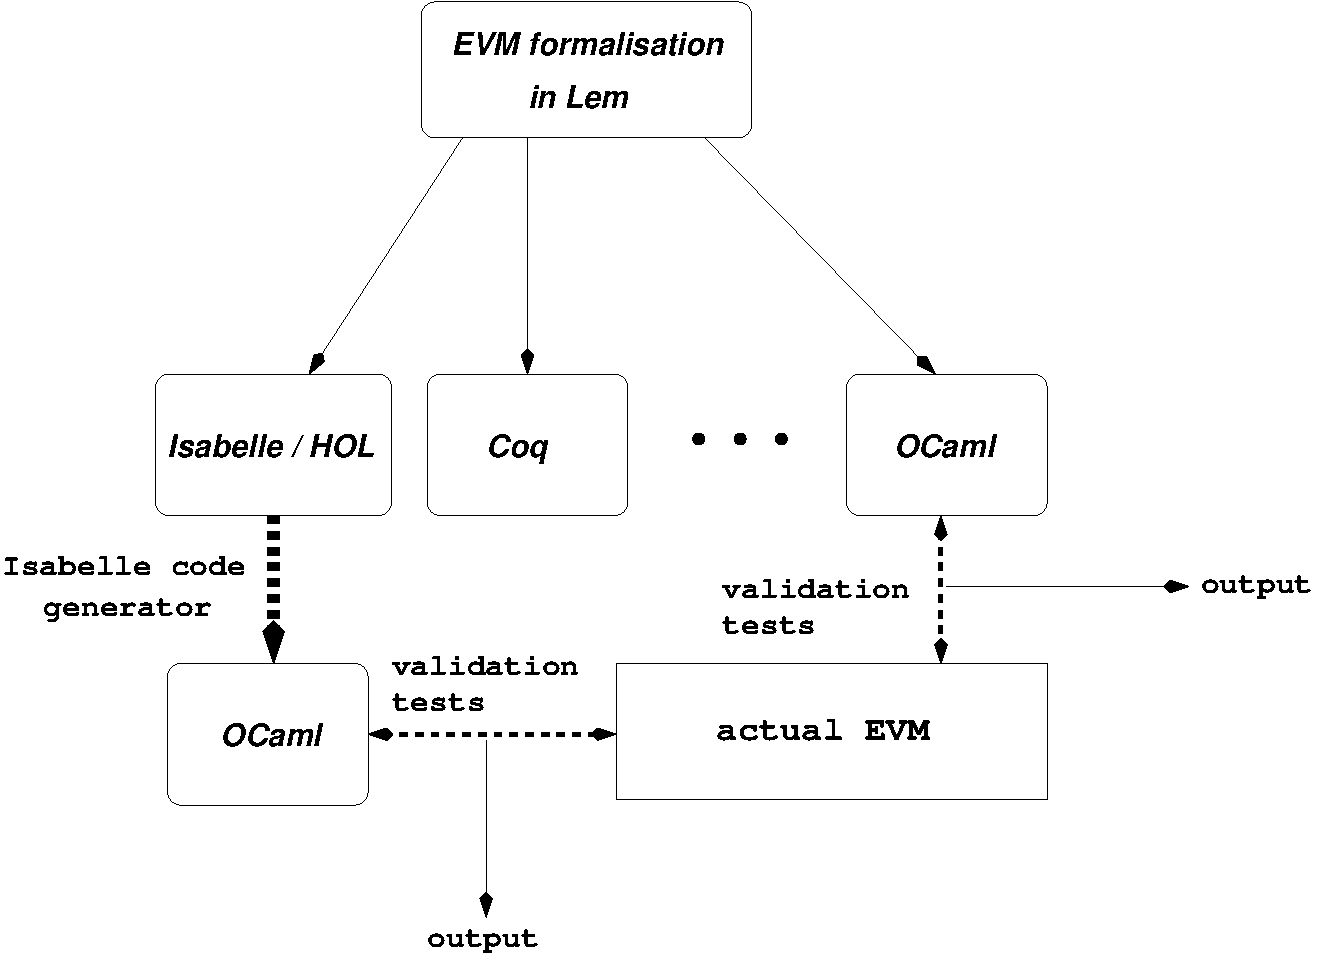
\includegraphics[height=5.5cm, width=7.5cm]{images/evm_lem}    
        \caption{Validation of EVM models.}
\label{fig:valid}
\end{figure}

Our `double-validation' process is outlined in Figure~\ref{fig:valid}.
The use of the test suite from Isabelle has required some effort, mainly because 
of different representations of machine words: OCaml code from Lem uses efficient native modules,
whereas the Isabelle side invokes a formally verified theory of machine words.
Because of this, our suite needs much more time to pass the tests.
Nonetheless, we gain a complementary indication that all three models of EVM follow the specification
and behave equally.    
%
\section{Total Correctness of EVM Bytecode Programs}
\label{sec:corr}
In his PhD thesis~\cite{DBLP:phd/ethos/Myreen09}, Myreen introduced a general 
method of formal verification of
machine code with a particular application to ARM. In this section we show how
this general method can be adapted to EVM, with additional consideration given to
EVM specific properties rooted in gas consumption.
 
In the general model, a state carries all the information needed to execute a program, including
instructions (with respective reference numbers) constituting the program itself, a program counter that
refers to the current instruction, a stack and so on. All these elements are treated uniformly 
as sets of so-called \emph{state elements}
and separated in a state using separation logic conjunctions $\sconj$ (denoted by $*$ in~\cite{Reynolds_02}).  
A single machine step is captured by a function $\xnext$ that 
takes the current instruction via program counter from the state and transforms the state in accordance with the instruction's
specified behaviour. Of course, $\xnext$ might not always be able to pick an instruction
as an execution can have terminated properly or with an exception. This is indicated within a state
by the $\ncont$ flag, which is just an abbreviation for the state element 
$\mathit{ContinuingElm}\:\mathit{False}$, 
as opposed to $\cont$ flag abbreviating $\mathit{ContinuingElm}\:\mathit{True}$. 
If $\ncont$ is present in a state, $\xnext$ leaves the state unchanged.   

A Hoare-style property of a program $c$ is captured by a triple
$\pvalid{P}{c}{Q}$, where $P$ and $Q$ are separation logic predicates on the state.
The triple is true iff for any state $s$ and predicate $F$ such that
\[
(P \sconj \code{c} \sconj F)\:s
\] 
holds, there exists a natural number $k$ such that 
\[
(Q \sconj \code{c} \sconj F)\:\xnext^k(s)
\] 
holds. The predicate $F$ is usually called in this context a \emph{frame}, 
and keeping it allows us to reason about parts of states locally. %using \emph{frame rule}(cf.~\cite{Reynolds_02}),
$\code{c}$ is another element specifying that the program code is present in the state, and
$\xnext^k$ denotes $k$-times iteration of $\xnext$.
Such triples %$\pvalid{P}{c}{Q}$ 
are highly generic and we cannot conclude much from many of these, except that
under given preconditions the program $c$ will pass a state satisfying $Q$. This changes immediately in cases where $Q$ is of
the form $\ncont \sconj Q'$, now stating that $c$ has reached a terminating state satisfying $Q'$.
Hence, showing $\pvalid{P}{c}{\ncont \sconj Q'}$ amounts to showing termination of the program $c$ in
a $Q'$-state.

This generic technique applies seamlessly to EVM programs as
shown by Hirai~\cite{Yoichi}.
However, we realised that showing termination of a contract individually is an unnecessary burden because
Ethereum was designed in such a way that all smart contracts
are guaranteed to terminate (either successfully or due to an `out-of-gas' exception).
More specifically, to ensure that miners get compensated for their costs
incurred by operating the Ethereum blockchain, each EVM instruction
has a gas fee.
When invoking a contract, the initiator provides a gas budget
proportional to how computationally expensive the execution is expected
to be and every step of execution is deducted from the budget.
If the gas consumption exceeds the budget, an `out-of-gas' exception is
raised,
the miner keeps all of the gas and
the state of the contract prior to the
invocation is restored.

These blockchain specifics give us a termination order. Thus, we 
augment the EVM formalisation~\cite{Yoichi} by the function $\xnext_\mu$ which 
consequently iterates $\xnext$ on each state as long as possible, i.e. the $\cont$ flag
is present.
%assigns to each state the first terminal state reachable via the 
%reflexive-transitive closure of $\xnext$. 
Hence, the essential property we show about $\xnext_\mu$ is that for any state $s$ there exists $k \geq 0$ such that
\begin{itemize}
\item[(i)] $\xnext_\mu(s) = \xnext^k(s)$ holds;
\item[(ii)] for any $l$, such that $0 \le l < k$, the state $\xnext^l(s)$ contains $\cont$;
%
%$\xnext$ can execute an instruction %continue 
%                          for any $l$ such that $0 \le l < k$
\item[(iii)] for any $l$, such that $l \ge k$, the state $\xnext^l(s)$ contains $\ncont$.
%cannot execute any instruction %continue                            
\end{itemize}
In other words, $\xnext_\mu(s) = \xnext^k(s)$ where $k$ is the least number such that
$\xnext^k(s)$ reaches a state with the $\ncont$ element. 
% Perhaps say that we proved that every program in EVM bytecode terminates by writing
% higher-order logic function that executes bytecode (reusing Yoichi's definitions of
% semantics) and proving termination of that function.

Now, regarding the contract correctness, we strengthen $\pvalid{P}{c}{Q}$ to 
a total input/output property $\tvalid{P}{c}{Q}$ which is true iff
for any state $s$ and frame $F$ 
\[
(P \sconj \code{c} \sconj F)\: s
\] 
implies 
\[
(Q \sconj \code{c} \sconj F)\: \xnext_\mu(s)
\] 
To sum up, what we achieved so far is to factor out the termination part which we have 
shown once and for all, thus removing this obligation from the verification
process completely. 

In the next section we will present our program logic processing EVM bytecode, 
which (based on soundness presented in Section~\ref{sec:sound}) will give us 
a sound device to derive verification conditions for contract properties of the form $\tvalid{P}{c}{Q}$.   
%
Although the program logic does not support general loops yet, factoring out the termination part
means that we would not need to provide any variants to establish loop properties since
gas consumption is a variant for any EVM-loop. On the other hand, we might then need to augment our triples
by an exception condition to handle cases when an `out-of-gas' exception is raised during
a loop iteration, thus not reaching the loop exit condition. Alternatively, we also might augment
any such condition by a check of remaining gas amount, such that any loop would just exit if not enough gas
is available to perform the next iteration. This approach would however require good approximations
of gas consumed per iteration.   
%
%       
\section{Program Logic}
\label{sec:logic}
A Hoare-style program logic comprises a collection of rules that allow us to derive semantic properties 
of compound programs from properties of its parts. In the case of structured languages 
we usually have, for instance, a rule telling us that a program \textbf{if} $C$ \textbf{then} $p_1$ \textbf{else} $p_2$
exhibits a certain input/output behaviour if $p_1$ and $p_2$ do so, however, with the additional precondition $C$ 
available for $p_1$ and $\neg C$ for $p_2$.
The situation is not that simple when we have to reason about EVM bytecode.
At this level, a conditional compound construct
appears merely as a jump instruction that transfers the flow of execution
to another part of the program.
In this sense, a program logic that treats the entire bytecode program simply as a list of instructions
would be in principle feasible, but intricate. 
%cannot solely rely on the structure of the program to
%guide formal reasoning, because the instruction following
%a jump is not necessarily next in the flow of execution.
%
%Although designing a logic that handles this would be in principle feasible,
%Since a bytecode program comprises
%a list of instructions, a rule might handle the head instruction and proceed to the tail of 
%the list, but would need to make exceptions when the head instruction is a jump, because then
%the tail does not necessarily correspond to the next instructions in the flow of execution.
%Although such treatment would be in principle feasible,
To this end more sophisticated techniques are available, such as decompilation via extraction of 
\emph{Control Flow Graphs} (CFG), in particular applied to the Java Virtual Machine (JVM) code~\cite{zhao99}.
The aim of CFG extraction is to split a program into \emph{basic blocks}, i.e. sequences of
instructions without jumps, and connect them
using edges corresponding to jumps.
The essential property of basic blocks is that
they comprise straight-line code, i.e. the control flow always enters it at its first instruction
and leaves only after the last one has been executed.
Thus, reasoning about bytecode at the CFG-level resembles reasoning about structured programs
in many aspects.
In particular, a CFG provides enough structure to add annotations,
such as loop invariants, enabling complete automation of the verification condition generation process.

%However, the algorithm to compute the edges of a CFG for JVM bytecode
%cannot be easily adapted to our EVM context.
However, full CFG extraction poses more advanced challenges in EVM context than for JVM,
especially from the formal modelling perspective.
This is because JVM jump instructions
take their target address as an immediate value argument which can be determined statically,
whereas in EVM jump destinations
must be obtained from the stack, i.e. dynamically. For that reason, our bytecode preprocessing
currently addresses basic block extraction only, presented in the next section.
Then, Sections~\ref{sec:prog-rules}, \ref{sec:block-rules} and \ref{sec:instr-rules} 
present how our logic handles programs, blocks and instructions, respectively. 
%
%       
%The basic blocks program logic we present in this section is organised
%in three levels of inductively defined inference rules, of the form:
%\[
%\begin{array}{l}
%\ttrip{\mathit{blocks}}{\mathtt{prog}}{P}{(n, \mathit{xs}, t)}{Q} \\
%\ttrip{}{\mathtt{block}}{P}{\mathit{xs}}{Q} \\
%\ttrip{}{\mathtt{instr}}{P}{\mathit{x}}{Q} 
%\end{array}
%\]
%where $P, Q$ are state predicates,
%$\mathit{blocks}$ is a list of basic blocks,
%$(n, \mathit{xs}, t)$ is a basic block,
%$\mathit{xs}$ is a list of instructions,
%and $x$ is an instruction.
%
%The program level allows considering one basic block at a time.
%The block level, one instruction at a time.
%And the instruction level provides rules for every instruction defined on the EVM.
%In the rest of this section we first explain in detail how we
%split EVM bytecode into basic blocks, then we dedicate a section to
%each level of the program logic.
%
\subsection{Extraction of Basic Blocks}
\label{sec:extract}
%
We divide EVM instructions into three groups:
\begin{itemize}
\item[(i)] $\instr{JUMPDEST}$ indicates a jump destination and hence beginning of a
                                 basic block;
\item[(ii)] $\instr{JUMP}$, $\instr{JUMPI}$, $\instr{UNKNOWN}$ and all of 
            \emph{Misc}-instructions\footnote{RETURN, STOP, SUICIDE, CREATE, CALL, CALLCODE, DELEGATECALL}
            indicate the end of a basic block ($\instr{UNKNOWN}$ and Misc-instructions interrupt program execution); 
\item[(iii)] all remaining instructions. %that form the contents of basic blocks.
\end{itemize}  
Furthermore, we classify basic blocks with the following four types:
\begin{itemize}
\item[(i)] \textit{Terminal} --- if the last instruction of the block interrupts execution;
\item[(ii)] \textit{Jump} --- if the last instruction is $\instr{JUMP}$;
\item[(iii)] \textit{Jumpi} --- if the last instruction is $\instr{JUMPI}$;
\item[(iv)] \textit{Next} --- otherwise, i.e. when control passes from the last instruction of the block
                             to the instruction with the successor address.                         
\end{itemize} 
\begin{figure}[ht!]
%\center
\begin{tabular}{c | r l | c}
                block index & address & instruction & block type\\
                        \hline
                {0}&       0       &       $\instr{OR}$&\textit{Next}\\
                &       1       &       $\instr{ADD}$&\\
                &    2       &       $\instr{SWAP1}$&  \\
                        \hline
                {3}&       3       &       $\instr{JUMPDEST}$&\textit{Jump}\\
                &       4       &       $\instr{MLOAD}$&\\
                &       5       &       $\instr{POP}$&\\
                &    \textcolor{gray}{6}     &       {\color{gray}$\instr{JUMP}$}& \\
                        \hline
                {7}&       7       &       $\instr{DUP3}$&\textit{Jumpi}\\
                &       8       &       $\instr{PUSH1}\;0$&\\
                &       10      &       $\instr{ISZERO}$&\\
                &    \textcolor{gray}{11}    &       {\color{gray}$\instr{JUMPI}$}& \\
                        \hline
                {12}&       12      &       $\instr{POP}$&\textit{Terminal}\\
                &   13      &       $\instr{RETURN}$& \\
                        \hline
        \end{tabular}
\caption{A program split into four basic blocks, where grey instructions appear in the original
         code but are removed from the list of instructions of their block.}
\label{fig:basicblocks}
\end{figure}
Figure~\ref{fig:basicblocks} illustrates how we split EVM bytecode into basic blocks of different
types, thereby indexing the blocks with addresses of their first instruction
and removing all the jumps from the block contents. %the list of instructions.
The entire extraction process is captured in the Isabelle development
by means of the function $\bblocks$ which maps a list of instructions to a list of tuples $(n, \mathit{xs}, t)$,
where $n$ is the block index, $\mathit{xs}$ is the list of instructions of the block, and $t$ is the type of
the block. 

By splitting bytecode into basic blocks no information gets lost since we can connect the produced blocks
in the right order and insert jumps back in accordance with block types. More precisely, we also have the function
$\cblocks$ such that for any bytecode program $c$ the identity 
\[
\cblocks(\bblocks\:c) = c
\]
holds.  

Based on these preparations, the following predicates 
for reasoning at different levels
will be defined inductively in the following three sections:
\[
\begin{array}{l l}
\ttrip{\mathit{blocks}}{\mathtt{prog}}{P}{(n, \mathit{xs}, t)}{Q} & 
\mbox{-- at the program level}\\
\\
\ttrip{}{\mathtt{block}}{P}{\mathit{xs}}{Q} &
\mbox{-- at the block level}\\
\\
\ttrip{}{\mathtt{instr}}{P}{\mathit{x}}{Q} &
\mbox{-- at the instruction level}
\end{array}
\]
where $P, Q$ are state predicates, $x$ is an instruction, $\mathit{xs}$ is a list of instructions,
$\mathit{blocks}$ is a list of basic blocks, and
$(n, \mathit{xs}, t)$ --- a basic block.% are defined inductively in the following three sections.
%
\subsection{Program Rules}
\label{sec:prog-rules}
%
We start at the program level, where we have the following rules for
each block type.
\[
\begin{array}{l l}
\mbox{(i)} & \RuleC{\ttrip{}{\mathtt{block}}{P}{\mathit{xs}}{Q}}
     {\ttrip{\mathit{blocks}}{\mathtt{prog}}{P}{(n, \mathit{xs}, \mathit{Terminal})}{Q}}
\end{array}
\]
That is, a $\mathit{Terminal}$-block is simply passed to the level of
blocks as we do not need to look at any other block after this has been processed.  

The rule for a $\mathit{Next}$-block is different in this respect:
\[
\begin{array}{l l}
\mbox{(ii)} & \RuleC{\begin{array}{l} \ttrip{}{\mathtt{block}}{P}{\mathit{xs}}{\pc\;m \sconj R} \\
                                      (m, \mathit{ys},t) \in \mathit{blocks} \\
                                       \ttrip{\mathit{blocks}}{\mathtt{prog}}{\pc\;m \sconj R}{(m, \mathit{ys},t)}{Q}
                     \end{array}}
     {\ttrip{\mathit{blocks}}{\mathtt{prog}}{P}{(n, \mathit{xs}, \mathit{Next})}{Q}}
\end{array}
\]
The state element $\pc\;m$ determines the program counter after $\mathit{xs}$ has been
processed. Then we need to retrieve the next block associated to the index $m$ from the structure $\mathit{blocks}$,
which is expressed by $(m, \mathit{ys},t) \in \mathit{blocks}$, and proceed with 
$(m, \mathit{ys},t)$.

Further, in case of a $\mathit{Jump}$-block we additionally need to retrieve the address of the jump 
destination from the stack 
after the block has been processed. This yields the following, slightly more involved, rule:
\[
\begin{array}{l l}
\mbox{(iii)} & \RuleC{\begin{array}{l}\ttrip{}{\mathtt{block}}{P}{\mathit{xs}}{R_1} \\
                                      (j, \mathit{ys},t) \in \mathit{blocks} \\
                                      \hd\mathit{ys} = (j, \instr{JUMPDEST}) \\
                                      \ttrip{\mathit{blocks}}{\mathtt{prog}}{R_2}{(j, \mathit{ys},t)}{Q}
                      \end{array}}
     {\ttrip{\mathit{blocks}}{\mathtt{prog}}{P}{(n, \mathit{xs}, \mathit{Jump})}{Q}}
\end{array}
\]
where $R_1$ and $R_2$ abbreviate the conditions \\
\\$
\begin{array}{l}
\pure{h \le 1023 \wedge g \geq 8} \sconj \cont \sconj \gaspred\:g \; \sconj \\
\pc\:i \; \sconj \stackh\:(h + 1) \sconj \stack\:h\:j \sconj R 
\end{array}
$\\ 
\\
and\\
\\$
\begin{array}{l}
\cont \sconj \gaspred\:(g - 8) \; \sconj \\
\pc\:j \; \sconj \stackh\:h \sconj R 
\end{array}
$\\
\\respectively. 
Regarding the stack, $\stackh\:(h + 1)$ and $\stack\:h\:j$ specify a state where
index $h$ refers to the top of the stack containing $j$ --- the jump destination we are looking for.
Regarding gas, $\gaspred\:g$
binds the available amount of gas to $g$, whereas 
the part $\pure{h \le 1023 \wedge g \geq 8}$ is a \emph{pure} condition,
i.e. not dependent on state, and sets an upper bound for the height of
the stack and a lower bound for the amount of gas, namely $8$ units: 
as much as EVM requires to perform a jump, which is deducted by $\gaspred\:(g - 8)$.   
Note that here and in the rules below we need to carry the $\cont$ state element because the EVM model~\cite{Yoichi}
imposes having either $\cont$ or $\ncont$ in a state to process instructions.
%Although the pure part is quite plain in this case, it generally allows us to express elaborated 
%conditions on state elements by means of higher-order logic formulae.      

The case of a conditional jump. i.e. a $\mathit{Jumpi}$-block, is similar, except
that we also need to retrieve from the stack the value $c$ to be compared to $0$ and
jump only if $c \neq 0$:
\[
\begin{array}{l l}
\mbox{(iv)} & \RuleC{\begin{array}{l l}\ttrip{}{\mathtt{block}}{P}{\mathit{xs}}{R_1} & \\
                                       (j, \mathit{ys},t) \in \mathit{blocks} & \\
                                       (i, \mathit{zs},t') \in \mathit{blocks} & \\
                                       \hd\mathit{ys} = (j, \instr{JUMPDEST}) & \\
  \ttrip{\mathit{blocks}}{\mathtt{prog}}{R_2}{(j, \mathit{ys},t)}{Q} & \bullet\; \mbox{if } c \neq 0 \\
  \ttrip{\mathit{blocks}}{\mathtt{prog}}{R_3}{(i, \mathit{zs},t')}{Q} & \bullet\; \mbox{if } c = 0 
                      \end{array}}
     {\ttrip{\mathit{blocks}}{\mathtt{prog}}{P}{(n, \mathit{xs}, \mathit{Jumpi})}{Q}}
\end{array}
\]  
where $R_1, R_2, R_3$ abbreviate the conditions \\
\\$
\begin{array}{l}
\pure{h \le 1022 \wedge g \geq 10} \sconj \cont \sconj \gaspred\:g \; \sconj \\
\pc\:(i - 1) \; \sconj \stackh\:(h + 2) \; \sconj \stack\:(h+1)\:j\; \sconj \\
 \stack\:h\:c \;\sconj R 
\end{array}
$\\ 
\\
and\\
\\$
\begin{array}{l}
\cont \sconj \gaspred\:(g - 10) \; \sconj \\
\pc\:j \; \sconj \stackh\:h \sconj R 
\end{array}
$\\
\\
and\\
\\$
\begin{array}{l}
\cont \sconj \gaspred\:(g - 10) \; \sconj \\
\pc\:i \; \sconj \stackh\:h \sconj R 
\end{array}
$\\
\\respectively. 
% 
\subsection{Block Rules}
\label{sec:block-rules}
At the level of basic blocks we need only two simple rules
that handle the cases of non-empty and empty lists of instructions
to be processed:
\[
\begin{array}{l l}
\mbox{(i)} & \RuleC{\begin{array}{l}\ttrip{}{\mathtt{instr}}{P}{x}{R} \\
                    \ttrip{}{\mathtt{block}}{R}{\mathit{xs}}{Q}
                    \end{array}}
                   {\ttrip{}{\mathtt{block}}{P}{x\mbox{::}\mathit{xs}}{Q}}
\end{array}
\]
and
\[
\begin{array}{l l}
\mbox{(ii)} & \RuleC{P \subpred Q} 
{\ttrip{}{\mathtt{block}}{P}{\mathit{Nil}}{Q}}
\end{array}
\]
where $P \subpred Q$ means $P\:s$ implies $Q\:s$ for any state $s$.
%
\subsection{Instruction Rules}
\label{sec:instr-rules}
To be able to verify any possible EVM bytecode program we need to provide a rule for 
each of 70 EVM instructions.
Presently we provide rules for 30 commonly used instructions,
and extend this set gradually `on-demand'.
However, the behaviour of instructions referring to the Ethereum global state, 
such as $\instr{CALL}$ for inter-contract calls, cannot be fully captured
by the EVM state alone.
As a result, in the EVM semantics (and accordingly in our logic) these
instructions lead to an environment action that must be modelled separately.
Such modelling is however possible and we discuss it further in Section~\ref{sec:concl}.

%
%Instructions such as $\instr{CALL}$, for inter-contract message calls, lead
%to an environment action that requires an appropriate model of the Ethereum global state,
%whereas the current EVM formalisation treats the global state merely as an unknown external environment.
%
%Our logic only allows reasoning about the EVM machine state,
%the rest of the Ethereum global state is treated as an external environment.
%Instructions such as $\instr{CALL}$, for inter-contract message calls, lead
%to an environment action that must be modelled separately.
%Such modelling is however possible and we discuss it further in Section~\ref{sec:concl}.
%
%, we will not
%present all of them here\footnote{We presently have
%proved the soundness of 30 commonly used instructions but
%we expect the missing instructions to follow a similar proof structure.}.
The following rule for $\instr{PUSH1}$, the operation pushing one byte on the stack, is quite representative
as it shows how we specify the necessary conditions for 
the instruction to be performed by the EVM in the precondition, as well as
the effect of the operation on state elements in the postcondition:
\[
\ttrip{}{\mathtt{instr}}{P}{(n, \instr{PUSH1}\:x)}{Q}
\]
where $P$ stands for 
\\
\\$
\begin{array}{l}
\pure{h \le 1023 \wedge g \geq 3} \sconj \cont \sconj \gaspred\:g \; \sconj \\
\pc\:n \; \sconj \stackh\:h \; \sconj F 
\end{array}
$\\ 
\\
and $Q$ for\\
\\$
\begin{array}{l}
\cont \sconj \gaspred\:(g - 3) \; \sconj \\
\pc\:(n+1) \; \sconj \stackh\:(h + 1) \sconj \stack\:h\:x \sconj F
\end{array}
$\\
\\
In particular, we have stated that the height of the stack increases by $1$ 
($\stackh\:(h + 1)$)
and that the top index $h$ of the stack points to the value $x$ ($\stack\:h\:x$)
among the effects of $\instr{PUSH1}$. It is also worth noting that we incorporate frames
into such instruction-specific rules by carrying a variable $F$ in pre- and
postconditions, as shown above. This is in contrast to the more common way, which is
introducing a generic \emph{frame} rule (cf.~\cite{Reynolds_02}) of the form
\[
\RuleC{\ttrip{}{\mathtt{instr}}{P}{i}{Q}}{\ttrip{}{\mathtt{instr}}{P \sconj F}{i}{Q \sconj F}}
\] 
and removing $F$ from all instruction-specific rules. Although the rule is sound, this treatment leads to 
a considerable overhead in the verification process, since we would need to apply
the frame rule each time an instruction-specific rule is applied. 
%For this practical reason we omit an explicit frame rule. 

Apart from the frame rule we still have two generic rules at the instruction level:
\[
\begin{array}{l l}
\mbox{(i)} & \RuleC{\begin{array}{l}
                     \ttrip{}{\mathtt{instr}}{P'}{i}{Q'} \\
                     P \subpred P' \\ 
                     Q' \subpred Q
                     \end{array}}{\ttrip{}{\mathtt{instr}}{P}{i}{Q}}
\end{array}
\]
\[
\begin{array}{l l}
\mbox{(ii)} & \ttrip{}{\mathtt{instr}}{\pure{\mathit{False}}}{i}{Q} 
\end{array}
\]
The rule (i) is the usual `consequence' rule, allowing us to adjust pre- and
postconditions, whereas (ii) is needed to discharge trivial 
proof obligations having unsatisfiable preconditions. Such obligations 
arise frequently from conditional jumps (rule (iv), Section~\ref{sec:prog-rules})
where the condition is fully evaluated prior to the actual jump, such that
we need to follow only one of the emerging branches.

The following section puts the program logic and the results of Section~\ref{sec:corr}
together by means of a soundness property and outlines its proof. 
%
\section{Soundness}
\label{sec:sound}
As our program logic is separated in three layers, we establish its soundness in three steps.

At the level of instructions, soundness basically amounts to the property
\begin{equation}
\label{prop:sound-instr}
\RuleC{\begin{array}{l}
         \ttrip{}{instr}{P}{x}{Q} \\
         (P \sconj \code{[x]} \sconj F)\: s
       \end{array}}
 {(Q \sconj \code{[x]} \sconj F)\: \xnext(s)}
\end{equation}
which we prove by structural induction on $\ttrip{}{instr}{P}{x}{Q}$. 
By this, we need to show that the pre- and postconditions, as specified in each 
rule for individual instructions, are indeed covered by the behaviour of 
the respective instruction. Note that $\code{[x]}$ ensures that 
$x = (\mathit{addr}, \mathit{instr})$ is present in the code-element of $s$, such that
$\xnext$ executes precisely the instruction $\mathit{instr}$, if $\pc\:\mathit{addr}$ is present in $s$ as well.
This, in turn, is obtained from the preconditions of instruction
rules, such as the $\instr{PUSH1}$-rule from the previous section.

Next, at the level of blocks we show
\begin{equation}
\label{prop:sound-block}
\RuleC{\begin{array}{l}
         \ttrip{}{block}{P}{\mathit{xs}}{Q} \\
         (P \sconj \code{\mathit{xs}} \sconj F)\: s
       \end{array}}
 {(Q \sconj \code{\mathit{xs}} \sconj F)\: \xnext^{\len{\mathit{xs}}}(s)}
\end{equation}
where the usage of $\xnext^{\len{\mathit{xs}}}$ is justified, since we consider
a basic block $\mathit{xs}$ which requires precisely $\len{\mathit{xs}}$ steps
to be processed completely.   
%
By induction on $\ttrip{}{block}{P}{\mathit{xs}}{Q}$ we need to consider the cases
when $\mathit{xs}$ is non-empty or empty.
In case $\mathit{xs} = x::\mathit{zs}$ we can assume $\ttrip{}{instr}{P}{x}{R}$
and $\ttrip{}{block}{R}{\mathit{zs}}{Q}$ such that 
\[
\RuleC{(R \sconj \code{\mathit{zs}} \sconj F)\: s}
 {(Q \sconj \code{\mathit{zs}} \sconj F)\: \xnext^{\len{\mathit{zs}}}(s)}
\]
holds by the induction hypothesis. 
Furthermore, from (\ref{prop:sound-instr}) and $\ttrip{}{instr}{P}{x}{R}$ we can further conclude 
\[
\RuleC{(P \sconj \code{[x]} \sconj F)\: s}
      {(R \sconj \code{[x]} \sconj F)\: \xnext(s)}
\]
which combined establish (\ref{prop:sound-block}).
Thereby we also make use of the equality
\[
\code{x::\mathit{zs}} = \code{[x]} \sconj \code{\mathit{zs}}
\] 
which holds since $x= (\mathit{addr}, \mathit{instr})$ does not occur in $\mathit{zs}$ due to
the unique $\mathit{addr}$.
 
Next, in case $\mathit{xs}$ is empty, we can assume $P \subpred Q$ which
immediately gives us (\ref{prop:sound-block}). 

The ultimate soundness statement is at the program level:
\begin{equation}
\label{prop:sound1}
\RuleC{\begin{array}{l}
       \ttrip{\bblocks\: c}{prog}{P}{\fblock}{Q} \\
       0 < \len{c} < 2^{256} 
       \end{array}}
{\tvalid{P}{c}{Q}}
\end{equation}
where $\fblock$ is a shorthand for the block with the smallest index in $\bblocks\: c$, and
the assumption $0 < \len{c} < 2^{256}$ is necessary to avoid dealing with empty programs
as well as programs with more than $2^{256}$ instructions (imposed by 
the design of EVM). In other words, in order to establish an input/output property specified by 
$\tvalid{P}{c}{Q}$, we can transform $c$ into its basic blocks $\mathit{bs}$, 
pick the first block $b$ from $\mathit{bs}$, and
apply the rules of our program logic to derive 
\[
\ttrip{\mathit{bs}}{prog}{P}{b}{Q}
\]

However, in order to show (\ref{prop:sound1}) we need some preparations to be able to apply
structural induction on the program logic rules. To this end we deploy our function $\cblocks$
and state the proposition
\begin{equation}
\label{prop:sound2}
\RuleC{\begin{array}{l}
       \ttrip{\mathit{bs}}{prog}{P}{b}{Q} \\
       b \in \mathit{bs}\\
       \wfblocks\:\mathit{bs}
       \end{array}}
{\tvalid{P}{\cblocks \: \mathit{bs}}{Q}}
\end{equation}
where $\wfblocks$ is our well-formedness predicate capturing all necessary technical details about block
structure, essentially retaining the property 
\[
\RuleC{0 < \len{c} < 2^{256}}
{\wfblocks(\bblocks \: c)}
\] 
for any program $c$. 

Thus, the proposition (\ref{prop:sound2}) is a generalisation of
(\ref{prop:sound1}), since for any $c$ we can instantiate $\mathit{bs}$ by $\bblocks \: c$ 
and $b$ by $\fblock$ in (\ref{prop:sound2}), and use the identity 
\[
\cblocks(\bblocks\:c) = c
\] 
from Section~\ref{sec:extract}.
to obtain (\ref{prop:sound1}). 

Unfolding the definition of $\tvalid{P}{\cblocks \: \mathit{bs}}{Q}$ in
(\ref{prop:sound2}) we further obtain
\begin{equation}
\label{prop:sound3}
\RuleC{\begin{array}{l}
       \ttrip{\mathit{bs}}{prog}{P}{b}{Q} \\
       b \in \mathit{bs}\\
       \wfblocks\:\mathit{bs} \\
      (P \sconj \code{\cblocks \: \mathit{bs}} \sconj F)\: s
       \end{array}}
{(Q \sconj \code{\cblocks \: \mathit{bs}} \sconj F)\: \xnext_\mu(s)}
\end{equation}
and can proceed by induction on $\ttrip{\mathit{bs}}{prog}{P}{b}{Q}$.
By this, we have to consider four cases: one for each type of the block $b$.
So, for instance, if $b = (n, \mathit{xs}, \mathit{Terminal})$, i.e. a terminal block,
we have $\ttrip{}{block}{P}{\mathit{xs}}{Q}$. 
Since $b$ is a part of the block list $\mathit{bs}$ by assumption, we can separate some $\mathit{bs'}$ 
such that 
\[
\begin{array}{l}
(P \sconj \code{\cblocks \: \mathit{bs}} \sconj F)\: s \quad = \\
(P \sconj \code{\mathit{xs}} \sconj \code{\cblocks \: \mathit{bs'}} \sconj F)\: s 
\end{array}
\] 
Hence, we can instantiate frame $F$ in (\ref{prop:sound-block}) by
\[
\code{\cblocks \: \mathit{bs}'} \sconj F
\]
and consequently obtain 
\[
(Q \sconj \code{\cblocks \: \mathit{bs}} \sconj F)\: \xnext^{\len{\mathit{xs}}}(s)
\]
As we consider a terminal block, the state 
$\xnext^{\len{\mathit{xs}}}(s)$ is the first one containing the $\ncont$ element, i.e.
\[
\xnext^{\len{\mathit{xs}}}(s) = \xnext_\mu(s)
\]
holds, concluding this case.

Although slightly more involved, the proof of the remaining three cases follows the
same principles,
making however additional use of the induction hypothesis.
%
\section{Case study}
\label{sec:case}

%To demonstrate the practicality of our program logic, we verify a smart contract.

% We provide the ground work to eventually get fully verified
% smart contracts. They will require reasoning about bytecode.
% Our framework could be used to have a formal connection
% between a  more structured language and bytecode.

Our development provides the ground work for full functional correctness
of Ethereum smart contracts.
These contracts are typically implemented in a high-level
language called Solidity.
In this case study, we demonstrate the practicality of our framework
by formally specifying and verifying properties of the bytecode 
generated by Solidity compiler from an escrow agreement smart contract.
Section \ref{sec:design} describes the design and implementation of
the contract; Section \ref{sec:spec}, its specification;
Section \ref{sec:verif}, its verification;
and Section \ref{sec:auto}, the machinery we developed
to maximize proof automation.

\subsection{Design and Implementation}
\label{sec:design}
%
We designed an escrow agreement smart contract for the Ethereum blockchain.
In our scenario, a \textit{buyer} wants to purchase a good from a \textit{seller}
but there is no particular reason to assume that they trust each other.
To this end both parties rely on an
escrow agent: an \textit{arbiter} they both trust. 
%% not sure what the commented sentence states and if we need it: 
%--- to achieve a safe transaction despite their potential mutual distrust.
In this agreement, the arbiter creates the contract specifying the
expected amount of Ether (the Ethereum crypto-currency), waits for the buyer to transfer the money to
the contract and decides whether to pay the seller or refund the buyer.
Apart from the arbiter's decision to pay or to refund, the purchase process
is governed by the smart contract.

\begin{figure}[h!]
\begin{lstlisting}[language=Solidity,escapeinside={@}{@},numbers=left]{}
contract Escrow {
@\label{lst:storevarbeg}@    address buyer;
    address seller;
    address arbiter;
@\label{lst:storevarend}@    uint256 amount;

@\label{lst:constbeg}@    function Escrow(address _buyer,
                    address _seller,
                    uint256 _amount) public {
@\label{lst:constbeg}@            require (amount > 0);
            buyer = _buyer;
            seller = _seller;
            arbiter = msg.sender;
@\label{lst:constend}@            amount = _amount;
    }

    function addfund() payable public  {
@\label{lst:addfundbeg}@        require (amount > 0 &&
                 msg.value == amount &&
                 msg.sender == buyer);
@\label{lst:addfundend}@        amount = 0;
    }

    function refund() public {
@\label{lst:refundbeg}@        require (amount == 0 &&
                 msg.sender == arbiter);
@\label{lst:refundend}@        selfdestruct(buyer);
    }

    function pay() public {
@\label{lst:paybeg}@        require (amount == 0 &&
                 msg.sender == arbiter);
@\label{lst:payend}@        selfdestruct(seller);
    }
}
\end{lstlisting}
\caption{Escrow smart contract allowing an arbiter to clear a
 transaction between two potentially distrusting parties.}
\label{solidity}
\end{figure}

\autoref{solidity} shows our implementation of the contract.
In Solidity, the functionality of a smart contract is encapsulated into a
\textit{contract interface} which has a well-defined interface with public and private elements, 
similarly to a class in object-oriented programming (OOP).
Creating a contract on the blockchain instantiates the contract interface.
Just like class instantiations in OOP, contracts are stateful objects
where \emph{storage variables} are stored on the blockchain.

Every variable declared as a member of a contract interface is
a storage variable, and hence persists across multiple invocations of the contract.
Lines \autoref{lst:storevarbeg}--\autoref{lst:storevarend} in \autoref{solidity}
declare variables carrying blockchain addresses of the three parties
involved in the agreement, as well as \textit{amount} that serves two purposes.
It not only stores
the amount of Ether for the purchase, but also enforces the order
in which the contract operations must be invoked.
%%%% Is this important somehow?
%It is stored in a 256-bit machine word, which is the
%native word size of the EVM.
%For this reason, Ethereum addresses that are 160-bit long
%are in practice also stored in 256-bit machine words.

The constructor part (lines \autoref{lst:constbeg}--\autoref{lst:constend})
is run by the Ethereum platform to initialise the contract when it gets deployed.
The environment variable \textit{msg} carries the information
about the Ethereum transaction that led to a contract deployment, 
including the address of the account that
sent the transaction (\textit{msg.sender}).
Solidity's built-in function \textit{require} throws an exception
if the specified condition evaluates to false.
In this case the transaction is basically rolled back, 
making only one exception with the amount of gas consumed so far, which
is retained. 

On line \ref{lst:constbeg}, we use \textit{require} to ensure that the arbiter creates
an escrow agreement with an amount greater than zero.
This condition is critical because \textit{addfund} (line \autoref{lst:addfundend})
expects \textit{amount} to be strictly positive,
before setting it to zero.
This way we guarantee that the buyer can only add the
funds expected to the contract once.
Note that \textit{msg.value} is an environment variable
storing the amount of Ether transferred as part of the transaction.

Further, \textit{addfund} is annotated with the keyword \textit{payable},
which indicates that this function is allowed to be invoked
by an Ethereum transaction along with a non-zero amount of
Ether.
By default, all contract functions are not payable
in order to prevent accidental loss of Ether.
The keyword \textit{public} indicates that
the function must be exported in the contract interface,
thus getting accessible for contract users.
For the Solidity compiler this means adding the function to the abstract binary
interface (ABI) and generating dispatch code to jump to this function within bytecode.
%to the appropriate function.
We describe the dispatcher further at the end of this section.

Only the buyer can successfully invoke \textit{addfund} and
the exact amount, as specified by the arbiter, must be transferred
along with the invocation.
%
Similarly, only the arbiter has been entitled to invoke the functions \textit{refund} (lines \autoref{lst:refundbeg}--\autoref{lst:refundend})
and \textit{pay} (lines \autoref{lst:paybeg}--\autoref{lst:payend}). 
Moreover, the \textit{amount} is required to be zero to this end, i.e.
the buyer must already have placed his fund in the contract. 
%are both protected such that they must be called by the arbiter,
%and so, after the buyer has placed the funds in the contract.
%The latter is enforced by checking that \textit{amount} is zero.
Both functions make use of the \textit{selfdestruct} built-in mechanism,
which transfers the totality of the funds held by the contract
to the address passed as argument, and subsequently destroys the contract.
%
\paragraph{Dispatcher}
%
When we compile a Solidity smart contract to EVM bytecode,
the compiler generates the contract interface
such that it adheres to its ABI specification.
The ABI specifies the signature of all the functions
available for a user of the contract.
The bytecode has single entry point (the first instruction),
and is passed a byte string as input, where the
first 32-bit word corresponds to a function identifier.
The identifier is a hash of the function signature
identifying which function of the contract must be invoked.
The piece of bytecode which compares the function identifier
to function hashes is called the \textit{dispatcher}.
The dispatcher is also responsible for unpacking function
arguments, and when no hash matches the function identifier,
it throws an exception.
The binary format for computing function hashes and
packing arguments is standardised so that contracts
written in various EVM languages can interoperate without
trouble.
Since the dispatcher is produced by the compiler, it is
invisible to a Solidity developer and must be verified at
bytecode level.

\subsection{Specification}
\label{sec:spec}

\begin{figure}[h]
\begin{lstlisting}[language=Isar]{}
definition 
  spec_Escrow :: [address, address, address,
                  address, 256 word, 32 word,
                  256 word]
                 \<Rightarrow> contract_action
where
  spec_Escrow sender buyer seller arbiter
              amount hash value =
 (if hash = addfund_hash \<and> sender = buyer \<and>
     value = amount \<and> amount > 0 then
    ContractReturn []
  else if hash = refund_hash \<and> sender = arbiter \<and>
          value = 0 \<and> amount = 0 then
    ContractSuicide buyer
  else if hash = pay_hash \<and> sender = arbiter \<and>
          value = 0 \<and> amount = 0 then
    ContractSuicide seller
  else
    ContractFail [ShouldNotHappen])

definition
  spec_amount :: [address, address, address,
                  256 word, 32 word, 256 word]
                 \<Rightarrow> 256 word
  spec_amount sender buyer seller amount
              hash value =
  (if hash = addfund_hash \<and> sender = buyer \<and>
      value = amount \<and> amount > 0 then
     0
   else
     amount)
\end{lstlisting}
\caption{Specification of a safety property of the Escrow smart contract.}
\label{spec}
\end{figure}

\autoref{spec} shows our handwritten specification of \textit{Escrow} in Isabelle/HOL,
including the functional correctness theorem we proved.
\textit{spec\_Escrow} is a definition used in the main theorem in \autoref{theorem} to specify
the return value expected by the contract.
The arguments have the same names as the storage variables or the environment
variables they carry the value for, except for \textit{hash} which corresponds
to the first 32-bit word of the input data byte string passed as argument
to the bytecode.

We obtain the constants \textit{addfund\_hash}, \textit{pay\_hash} and
\textit{refund\_hash} from the ABI information generated by the Solidity compiler.
At a high-level, the specification says that the contract can
terminate in one of these four ways:
(1) it only return successfully when \textit{addfund}
is invoked with the right amount by the buyer;
all the funds will be fully returned via self-destruction of
the contract to either, (2) the buyer,
(3) or the seller;
(4) any other input leads to an exception denoted by \textit{ContractFail [ShouldNotHappen]}.

Note that the amount transferred via \textit{ContractSuicide} corresponds
to the balance of the contract stored in the Ethereum global state and
is unrelated to the value stored in the \textit{amount} storage variable
when the contract is destroyed.

In addition to specifying the return action of the contract, we want
to guarantee that \textit{addfund} can only be called once.
This is done with the \textit{spec\_amount} definition which
is used in the main theorem to specify the value of the
\textit{amount} storage variable.
It says that when the precondition for \textit{addfund} to
return successfully is met, \textit{amount} is set to zero,
thus protecting against further invocations of \textit{addfund}.

\begin{figure}[h]
\begin{lstlisting}[language=Isar]{}
theorem verify_escrow:
 \<exists>r. \<models> [pc 0 \<and>* stack_height 0 \<and>*
        sent_data (word_rsplit hash) \<and>*
        sent_value v \<and>* caller sender \<and>*
        memory_usage 0 \<and>* continuing \<and>*
        gas_pred 100000 \<and>* 
        storage 0 (ucast buyer) \<and>*
        storage 1 (ucast seller) \<and>*
        storage 2 (ucast arbiter) \<and>*
        storage 3 (ucast amount) \<and>*
        ... ]
         (build_blocks bytecode_Escrow)
       [action (spec_Escrow sender buyer seller
                  arbiter amount hash v) \<and>*
        storage 0 (ucast buyer) \<and>*
        storage 1 (ucast seller) \<and>*
        storage 2 (ucast arbiter) \<and>*
        storage 3 (spec_amount sender buyer
                     seller amount hash v) \<and>*
        r]
\end{lstlisting}
\caption{The correctness statement in our program logic.}  
%\caption{Functional correctness theorem of the Escrow smart contract.}
\label{theorem}
\end{figure}

Finally, the main theorem in \autoref{theorem} states the input/output 
property we proved.
It has the form of Hoare triples introduced in Section~\ref{sec:corr}.
The precondition initialises the machine state, e.g. program counter is $0$,
stack is empty, etc.
Importantly, \textit{hash} is the 32-bit word contract
argument used by the dispatcher code as well as the specification.
We convert it into a string of bytes to form the input data of the contract
using \textit{word\_rsplit}.
$\gaspred$ specifies the gas budget for the execution and $\storage$
binds storage entries to the free variables \textit{buyer}, \textit{seller},
\textit{arbiter} and \textit{amount}, initialised by the constructor.
Using \textit{ucast}, we convert 160-bit words representing Ethereum
addresses into the storage unit, which is 256-bit word.
\textit{bytecode\_Escrow} is a list of deeply embedded EVM
instructions which we convert into a list of basic blocks with $\bblocks$.
In the postcondition, we are only interested in the resulting action
satisfying \textit{spec\_Escrow}, storage variables being unchanged
and \textit{amount} corresponding to \textit{spec\_amount};
hence we quantify existentially on the rest of the state \textit{r}
to leave it unspecified.

\subsection{Verification}
\label{sec:verif}
Smart contract bytecode is divided into two sections: the pre-loader and
runtime code.
The pre-loader bootstraps the contract by deploying it on the
Ethereum network and running its constructor.
The runtime code only contains the core functionality of the contract
that can be invoked by other blockchain agents.
Our verification considers only the runtime code of \textit{Escrow},
thus excluding its constructor.

We obtain the runtime code as a byte string of hexadecimal opcodes
from the Solidity compiler and convert it into a list of EVM instructions via an
Isabelle/HOL function.
In this sense we work directly on the bytecode output of
the Solidity compiler.

\textit{Escrow} bytecode has 191 EVM instructions, that get split into 45 basic
blocks, including 12 of type \textit{Jumpi} (i.e.\ conditional jumps),
23 \textit{Terminal}, 6 \textit{Next} and 4 \textit{Jump}.
Once the automation support described in the next section reached maturity,
proving correctness of the bytecode was rather a routine task. %fairly straightforward

Some creativity was required to handle all the cases where the
contract ends with an exception.
The existential variable in the postcondition of our correctness
statement means that we have to provide a witness for the
unspecified part of the state.
The witness is automatically constructed by running our
proof automation tactics, however, for this to work the
existential variable must remain a unification variable until
we reach a \textit{Terminal} basic block.
The \textit{Terminal} block rule replaces the
unification variable with a concrete value,
so to ensure that each path gets a new unification
variable, we manually distinguish each case in the proof.

A difficult proof arose when parsing the contract input data
in order to extract the argument passed to the dispatcher.
This involved dealing with operations on words of different size,
which is notoriously hard.
In particular, the instruction $\instr{CALLDATALOAD}$ reads a
256-bit machine word from the input data array.
Since the hash value passed in the input data is only a 32-bit word,
the dispatcher does the following word arithmetic to convert the value:
\[
\mathit{w32}\mbox{-}\mathit{hash} = (\mathit{w256}\mbox{-}\mathit{input}\mbox{-}\mathit{data} \gg 224)\ \text{\&}\ \mathtt{0xffffffff}
\]
With the help of Isabelle's machine word library~\cite{Word_Lib-AFP},
we proved that when the hash is packed in the input data,
the above bit-wise operations return the same hash value.

%% mole $ wc -l HoareTripleForBasicBlocks.thy SoundnessForBasicBlocks.thy ../example/Dispatcher.thy ../EvmFacts.thy Hoare.thy
%%    575 HoareTripleForBasicBlocks.thy
%%   2733 SoundnessForBasicBlocks.thy
%%    762 ../example/Dispatcher.thy
%%    300 ../EvmFacts.thy
%%   1077 Hoare.thy
%%   5447 total

The total development of our framework is $\approx$6000 lines of Isabelle/HOL theories,
excluding the existing formalisation of EVM model, etc.
The size of the top-level specification of \textit{Escrow} is $\approx$30 lines
and the functional correctness proof of the contract is
$\approx$40 lines of proof specific to this example, which compares
favourably with the $\approx$500 lines of reusable proof
automation machinery we developed.
We describe this automation next.



% focus on runtime binary, 
% parse_bytecode 
% derivation tree for bytecode, 
% word proofs

% due to hash_in_w256 being padded with zeros,
% we need to prove hash_in_w32 = (hash_in_w256 >> 224) & 0xffffffff
% >> 224 removes the padded zeros
% Word proofs are notorious to be hard and this was one of them.

\subsection{Automation}
\label{sec:auto}
% Ideas: show isabelle tactics,
% number of lines of proofs
%
When reasoning about bytecode, even the verification of small contracts
can involve long, tedious and repetitive proofs.
Hence, our program logic was purposefully designed to be
amenable to proof automation.

The inductively defined inference rules, presented in Section~\ref{sec:logic},
are designed to be used in a syntax-driven verification
condition generator (VCG).
Shaping the rules in a way that the conclusion of at most one of them
can match the subgoal at each point in the
proof makes it easy to write a VCG that just tries applying all of the rules
one after another.
This tactic can be implemented with a few lines of Eisbach~\cite{Matichuk_MW_16} ---
Isabelle/HOL's high-level tactic language.
We developed a VCG for each level of our program logic.
For instance, the program-level tactic looks as follows:
\begin{lstlisting}[language=Isar]{}
method prog_vcg =
 (prog_jumpi_vcg | prog_jump_vcg
 | prog_terminal_vcg | prog_next_vcg)+
\end{lstlisting}
where e.g., \textit{prog\_jumpi\_vcg} is another tactic applying the \textit{Jumpi}-rule (iv) 
in Section~\ref{sec:prog-rules} and solving its resulting subgoals by
invoking more specific tactics we designed.
Altogether, \textit{prog\_vcg} tries each of the tactics separated by the $|$ symbol,
whereas the $+$ sign at the end means that it will do that repetitively until
none of the tactics is applicable. 

A common source of friction we experienced during the early development phase
of our framework was with proving goals of the form:
$\forall s.\: R\:s \longrightarrow P\:s$ where $P$ and $R$ are separation logic predicates
comprising the same separation conjunctions but in different orders.
Such proof obligations arise when we weaken a precondition to be
able to apply an $\vdash_\mathtt{instr}$ rule.
Since each $\vdash_\mathtt{instr}$ rule expects a separation logic expression with conjunctions
in a specific order, we routinely have to reorder these to
match a given precondition.

To ease the pain, we reuse the separation logic algebra framework~\cite{Klein_KB_12},
which provides a set of generic Isabelle tactics to manipulate separation logic terms.
We instantiated the algebra with the EVM machine state and created Isabelle tactics
which reorder separation conjunctions such that, e.g. %%% why e.g. ? 
the first term in $P$ matches the first one of $R$.
Once the first elements match, we leverage the tactics of the separation
algebra framework to remove the first element from both $R$ and $P$.

An issue we encountered is that when $R$ contains variables,
we have to reorder terms in $P$ in such way that the variables in $R$ get instantiated
in the correct order.
%%%
When such problem occurs, we resort to manual reordering of terms. % ?? 
%
\section{Related Work}
\label{sec:rwork}
%
As a consequence of the repeated exploitation of security flaws in smart contracts,
a notable amount of approaches and tools have already been proposed (e.g.~\cite{Bhargavan:2016:FVS:2993600.2993611,securify,Luu_COSH_16}).
 
The major trend is to apply various kinds of static analysis not only at the level of structured contract
languages (e.g. Solidity's Why3 backend~\cite{filliatre2013why3,Reitwiessner_16}) but also at the bytecode level~\cite{Msuiche_17,securify,Luu_COSH_16}. 
%However, most tools do not provide a lot of insight into internal details.
%
The obvious advantage of static analysis approaches is that full automation can be achieved for 
contract properties that can be confirmed statically, e.g. certain orders of transactions \cite{securify}.
The tools Oyente~\cite{Luu_COSH_16} and Porosity~\cite{Msuiche_17} decompile
bytecode into a control flow graph and perform control flow analysis in order
to detect common smart contract security defects such as re-entrancy bugs.
These tools are of great value when added to the development process so
they can unveil mistakes in early stages, but they do not prove functional correctness.

Our approach is more general as we aim to specify and verify contract properties in pre/postcondition
style where the conditions can comprise any higher-order logic formula describing an EVM state. 
For that reason, the degree of automation is limited in our case such that the user will need to interact 
with the proof system to discharge elaborated claims.

Bhargavan et al.~\cite{Bhargavan:2016:FVS:2993600.2993611} proposed a technique using an
intermediate functional language called $F^*$,
which is more amenable to verification. 
It provides not only translation of a subset of Solidity programs 
to $F^*$, but also decompilation of EVM bytecode to $F^*$ as well.
This use of decompilation makes
the approach similar to ours, since our program logic, in fact, resembles decompilation.
As explained in Section~\ref{sec:logic}, we split bytecode program into blocks without jumps
and determine the actual jump destinations dynamically `on-the-fly', by applying logic rules.
By contrast, Bhargavan et al. perform static stack analysis to this end.
However, a more striking difference is that our approach is homogeneous since every step of our verification process 
is performed and justified within a single, trusted logical framework without any translations to or from other formalisms.
Such translations must be either assumed to behave correctly in some sense or
formally modelled and verified, whereas we aimed to avoid both of these options.

KEVM~\cite{Hildenbrandt_SZRDGR_17} is a formal semantics of the EVM written using the K-framework.
Like the Lem semantics~\cite{Yoichi} we use, KEVM is executable and therefore can run the Ethereum foundation's validation test suite.
Reasoning about KEVM programs involves specifying properties in Reachability Logic and
verifying them with a separate analysis tool.
K supports translation for analysis with tools of varying
power, including symbolic execution, faster concrete execution, or Isabelle.
As explained earlier, we preferred the option of working in a single trusted logical framework.

%% Hirai~\cite{Yoichi} developed a Hoare logic for EVM bytecode
%% in the line of Myreen's work~\cite{DBLP:phd/ethos/Myreen09}.
%% In some sense, our work extends Hirai's by forcing Hoare triples to
%% state total correctness and by extracting a more structured representation
%% of the bytecode with basic blocks.
%% The restored structure of the bytecode facilitated the design of
%% a sound program logic and ultimately enabled more proof
%% automation as explained in Section~\ref{sec:auto}.

% XCAP ?

\section{Conclusions and Future Work}
% Ideas: inter-contract communication, recovering loops, more structured
% programs including notion of contract classes etc, CakeML backend, Jinja backend
% verification contract creation code, as opposed to run-time code.
\label{sec:concl}
In this paper we have presented our approach to the verification of Ethereum smart contracts
at the level of EVM bytecode. Building strictly on the thoroughly validated formal EVM model~\cite{Yoichi} in Isabelle/HOL,
we have augmented it using the fact that EVM gas consumption allows us to state properties of contracts in pre/postcondition style
with all termination considerations discharged. Further, we have outlined how we split contracts into a
structure of basic blocks as well as how a sound program logic proceeds from such blocks down to the level of instructions. 
The presented case study has demonstrated the applicability of our
program logic to real bytecode, verifying dispatch code that exhibits a structure
that appears in a similar form
in each Solidity-generated bytecode program. 
Moreover, the case study outlined how we use Isabelle tactics to automate
large parts of verification condition generation process.

To further foster formal verification of Ethereum smart contracts, we
could restore more of Solidity's control structures as well as function calls.
For instance, restoring loops would require using heuristics
to detect them and the program logic would be proved sound only
for the subset of EVM bytecode accepted by this heuristic.
Similarly detecting function calls in EVM bytecode requires
complex stack analysis because the EVM provides no support to call
subroutines and for stack unwinding.
Thus, heuristics must be used to distinguish call sites and
stack unwinding from other stack-manipulating instructions.
However, the proposal~\cite{subroutines} (\emph{EVM1.5}) is currently being discussed and 
suggests adding static jumps as well as instructions to call and
return from sub-routines (internal functions) to the EVM instruction set.
If implemented, it would greatly facilitate
decompilation and reasoning about EVM bytecode, as most of the aforementioned
issues would go away.

As mentioned in Section~\ref{sec:instr-rules}, our framework currently does not support reasoning about inter-contract message calls.
%reasoning outside the program logic.
When a contract $A$ makes a message call to contract $B$,
the execution of $A$ terminates in our formal model with a \textit{ContractCall} action.
Hence, within our program logic we can only prove properties
about the state of $A$ right before it calls $B$.
To reason further about such interactions, the Ethereum global state %environment
must be modelled separately to capture the behaviour of $B$.
For example, Hirai~\cite{Yoichi} has extended his framework,
on which ours is based, to formally verify that a smart contract
throws an exception if it is subject to a re-entrant invocation
($B$ attempts to call $A$).
As a future work, we could imagine an EVM formalisation parameterised by
a contract environment which directly invokes the target contract
when a message call occurs.

Another promising avenue for research is certifying compilers.
We believe that the Ethereum community
would greatly benefit from an EVM backend for the CakeML~\cite{Owens_NKMT_17}
verified compiler.
Since CakeML is a functional programming language, it would
provide a different approach to specification and verification of high-level properties
of smart contracts.
% compared to reasoning about bytecode directly.
%Yet the compiler correctness proof would imply the
%same level of guarantee as bytecode verification.


%% Acknowledgments
%% Yoichi Hirai, Corey Lewis, Peter H\"ofner 

\begin{acks}                            %% acks environment is optional
                                        %% contents suppressed with 'anonymous'
  %% Commands \grantsponsor{<sponsorID>}{<name>}{<url>} and
  %% \grantnum[<url>]{<sponsorID>}{<number>} should be used to
  %% acknowledge financial support and will be used by metadata
  %% extraction tools.
%  This material is based upon work supported by the
%  \grantsponsor{GS100000001}{National Science
%    Foundation}{http://dx.doi.org/10.13039/100000001} under Grant
%  No.~\grantnum{GS100000001}{nnnnnnn} and Grant
%  No.~\grantnum{GS100000001}{mmmmmmm}.  Any opinions, findings, and
%  conclusions or recommendations expressed in this material are those
%  of the author and do not necessarily reflect the views of the
%  National Science Foundation.


We would like to thank Yoichi Hirai, Corey Lewis, Peter H\"ofner
and Paul Rimba for all comments and suggestions.
\end{acks}


%% Bibliography
\bibliography{evm}


%% Appendix
%\appendix
%\section{Appendix}
%Text of appendix \ldots

\end{document}
